\chapter{Historia térmica, última dispersión y sopa primordial}

\lectureoverview{La historia de expansión del universo es también una historia térmica. Empezamos definiendo la temperatura mediante el equilibrio y el equilibrio mediante la dispersión. Un gas de fotones adquiere el espectro de Planck mientras las cargas libres lo mantienen en equilibrio térmico; cuando los electrones se unen a los protones, la radiación se desacopla, pero conserva su forma de cuerpo negro mientras todas las longitudes de onda se estiran con el factor de escala. La enorme proporción de fotones respecto de la materia explica entonces por qué la recombinación ocurre a una temperatura muy inferior a la de ionización del hidrógeno. Al retroceder aún más, pasamos por la última dispersión, la igualdad entre materia--radiación, el equilibrio de pares electrón--positrón y, finalmente, el pequeño exceso de materia--antimateria que sobrevive a la aniquilación.}

\section{Del ajuste de modelos a la historia térmica}

Un modelo cosmológico queda especificado, como mínimo, por la historia del factor de escala y la geometría espacial,
\begin{equation}
a(t),
\qquad
k\in\{+1,0,-1\}.
\end{equation}
El método práctico consiste en elegir el modelo, calcular sus predicciones, compararlas con los datos y ajustar los parámetros. También es posible invertir directamente la inferencia a partir de los datos, pero a menudo resulta menos transparente.

Es difícil determinar la curvatura a partir de fuentes relativamente cercanas. Así como la curvatura de la Tierra es una pequeña corrección a lo largo de una distancia terrestre corta, la curvatura espacial tiene un efecto débil cuando la distancia cosmológica no es suficientemente grande. Esto es tanto una desventaja como una ventaja: los estudios ordinarios de fuentes no determinan con precisión \(k\), pero una incertidumbre moderada en \(k\) no impide reconstruir de manera útil la historia de expansión.

Dos familias de observables aportan gran parte de la información. Las candelas estándar proporcionan el brillo en función del corrimiento al rojo, mientras que los estudios de fuentes proporcionan el número de objetos en un intervalo de corrimiento al rojo. Los ajustes resultantes favorecen una historia de expansión con una contribución sustancial de energía del vacío. Para obtener información precisa sobre la curvatura se necesita el brazo de palanca geométrico mucho mayor que proporciona el fondo cósmico de microondas.

Ahora cambiamos de pregunta. En lugar de preguntar solo cómo evoluciona \(a(t)\), preguntamos cómo evoluciona la temperatura del universo. Para empezar, planteamos una pregunta más elemental: ¿en qué condiciones tiene temperatura un sistema?

\section{Cuándo tiene temperatura un universo}

La temperatura es una propiedad del equilibrio térmico. Un conjunto de partículas se aproxima al equilibrio mediante colisiones, que deben ocurrir más rápido de lo que cambia el entorno macroscópico. En un universo en expansión, la comparación útil es
\begin{equation}
\tau_{\rm scatt}\ll H^{-1},
\label{eq:c07-equilibrium-condition}
\end{equation}
donde \(\tau_{\rm scatt}\) es un tiempo característico entre dispersiones y \(H^{-1}\) es el tiempo de expansión. Cuando esta desigualdad deja de cumplirse, el universo cambia antes de que las colisiones puedan restablecer el equilibrio.

Consideremos una caja con paredes perfectamente reflectantes. Dirijamos hacia ella un pulso láser, cerremos la abertura y supongamos que solo contiene fotones. El pulso rebota indefinidamente, pero los fotones ordinarios de baja energía se dispersan entre sí con una intensidad extraordinariamente débil. La reflexión por sí sola no redistribuye su energía hasta producir un espectro térmico. Por tanto, un gas de fotones no se termaliza por el mero hecho de estar confinado.

Las partículas con carga libres cambian la situación. Una onda electromagnética acelera un electrón; la carga acelerada vuelve a emitir radiación, de modo que los fotones se dispersan con eficiencia. Si hay suficientes electrones y protones libres, las dispersiones repetidas redistribuyen la energía entre las tres especies hasta que forman una sola sopa térmica con una temperatura común.

A gran escala, el universo es eléctricamente neutro. En la contabilidad más sencilla,
\begin{equation}
n_{e^-}=n_p,
\label{eq:c07-neutrality}
\end{equation}
porque las cargas del electrón y del protón tienen la misma magnitud y signos opuestos. Esta ecuación expresa la neutralidad; no explica por qué el universo es neutro ni por qué coinciden las magnitudes de ambas cargas. Esos son hechos más profundos de la física de partículas.

La distinción entre un plasma y un gas neutro es decisiva. Los electrones libres dispersan la radiación con eficiencia. Una vez que los electrones se unen a los protones para formar hidrógeno neutro, los campos eléctricos dominantes se cancelan a grandes distancias y la dispersión se vuelve mucho menos eficaz. A la baja densidad del universo actual, la materia neutra no puede llevar los fotones de fondo al equilibrio en el transcurso de una edad cósmica.

A una temperatura suficientemente alta, las colisiones energéticas ionizan el hidrógeno repetidamente y mantienen una población considerable de cargas libres. Los electrones, los protones y los fotones comparten entonces una misma temperatura. Al enfriarse el sistema, los átomos sobreviven, la densidad de electrones libres cae drásticamente y se pierde el equilibrio común. Las temperaturas que después se asignan a la materia y a la radiación no tienen por qué coincidir.

\begin{classroomqa}
\audiencequestion{Si el fondo de microondas tiene hoy una temperatura cercana a \(3\,\mathrm{K}\), ¿es esa la temperatura de todo el universo?}
\lecturerresponse{No. El espectro de los fotones puede describirse mediante una temperatura de cuerpo negro, pero la materia actual no está en equilibrio con esos fotones. Los distintos componentes tienen temperaturas cinéticas o efectivas diferentes, por lo que hoy no existe una única temperatura termodinámica global.}
\end{classroomqa}

\section{Radiación térmica y el giro cuántico}

Un campo de radiación en equilibrio contiene un espectro de longitudes de onda y frecuencias relacionadas por
\begin{equation}
\nu\lambda=c.
\end{equation}
Para no confundir la radiancia con la densidad de energía, denotemos mediante \(u_\nu(T)\) la energía por unidad de volumen y por unidad de frecuencia:
\begin{equation}
dE=u_\nu(T)\,dV\,d\nu.
\label{eq:c07-spectral-density}
\end{equation}
Así, \(u_\nu\) tiene dimensiones de energía dividida por volumen y frecuencia.

La temperatura misma es una escala de energía. Las unidades históricas de temperatura ocultan este hecho, por lo que la constante de Boltzmann proporciona la conversión:
\begin{equation}
E_{\rm thermal}\sim k_B T.
\end{equation}
Se puede tomar \(k_B=1\) en unidades naturales, pero conservarla permite distinguir claramente los kelvin de la energía.

Antes de la mecánica cuántica, el análisis dimensional basado en \(k_BT\), \(\nu\) y \(c\) da la densidad espectral de energía de Rayleigh--Jeans,
\begin{equation}
u_\nu^{\rm RJ}(T)=\frac{8\pi\nu^2}{c^3}k_BT.
\label{eq:c07-rayleigh-jeans}
\end{equation}
El factor numérico depende del recuento de los modos electromagnéticos, pero el comportamiento clásico esencial es \(u_\nu\propto T\nu^2\). Crece sin límite al aumentar la frecuencia y, por tanto, predice
\begin{equation}
\int_0^\infty u_\nu^{\rm RJ}\,d\nu=\infty.
\end{equation}
Este resultado imposible es la catástrofe ultravioleta. En cambio, el espectro medido primero aumenta, alcanza un máximo y luego cae con suficiente rapidez para que la energía total sea finita.

La constante de Planck introduce la escala cuántica que faltaba. Para la densidad espectral de energía definida en la ecuación~\eqref{eq:c07-spectral-density}, la ley de Planck es
\begin{equation}
u_\nu(T)
=
\frac{8\pi h\nu^3}{c^3}
\frac{1}{e^{h\nu/(k_BT)}-1}.
\label{eq:c07-planck}
\end{equation}
El exponente depende de la razón adimensional
\begin{equation}
x=\frac{h\nu}{k_BT},
\end{equation}
porque \(E_\gamma=h\nu\) y \(k_BT\) son ambas energías.

A bajas frecuencias, \(x\ll1\), y
\begin{equation}
e^x-1=x+O(x^2).
\end{equation}
Al sustituir en la ecuación~\eqref{eq:c07-planck} se obtiene
\begin{align}
u_\nu(T)
&\simeq
\frac{8\pi h\nu^3}{c^3}
\frac{k_BT}{h\nu}
\\
&=
\frac{8\pi\nu^2}{c^3}k_BT,
\end{align}
Así se recupera la física clásica en su dominio correcto de bajas frecuencias. A altas frecuencias, \(x\gg1\), el término exponencial domina y suprime el espectro. La transición ocurre cuando
\begin{equation}
\frac{h\nu}{k_BT}\sim1.
\label{eq:c07-crossover}
\end{equation}
Este es el punto en que la caída cuántica sustituye al crecimiento clásico.

\begin{figure}[htbp]
\centering
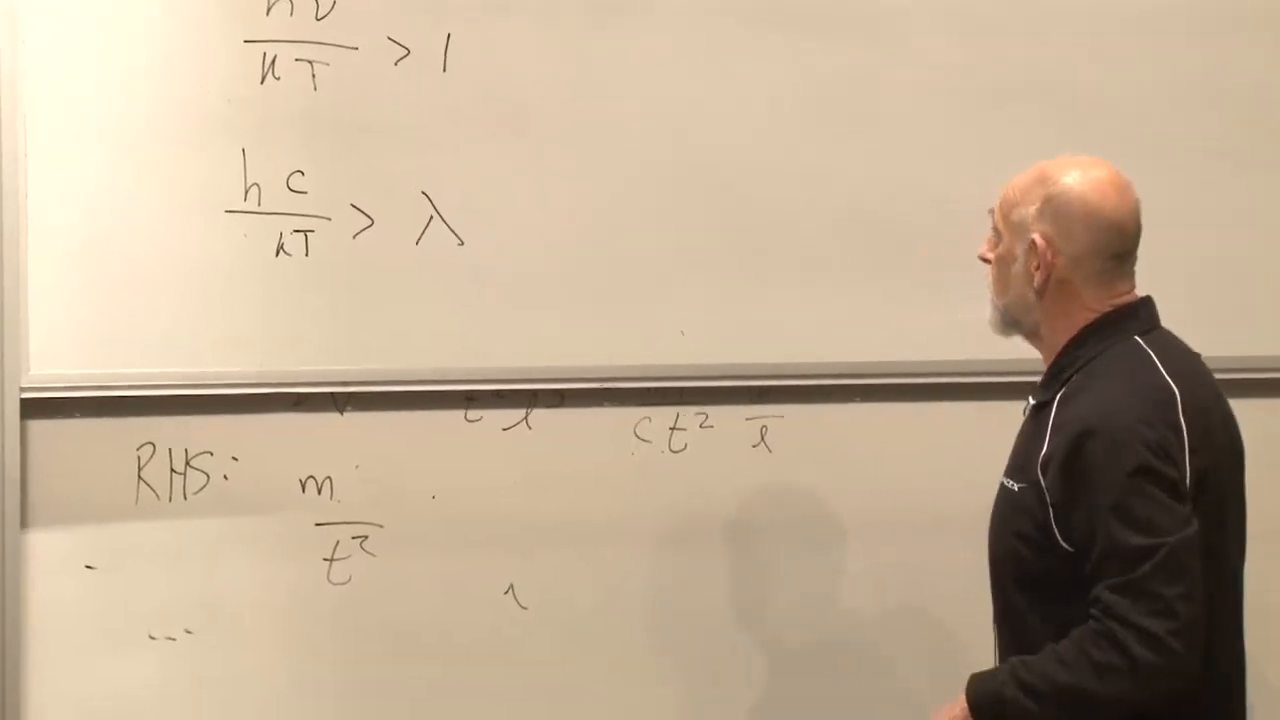
\includegraphics[width=0.82\textwidth]{lecture_07_figure_02.png}
\caption{La transición térmica en la pizarra. La expresión recortada de la parte superior es \(h\nu/(kT)>1\), y la expresión inferior, claramente visible, es \(hc/(kT)>\lambda\). Los restos tenues de la parte inferior de la pizarra no se usan como evidencia de las ecuaciones.}
\label{fig:c07-thermal-board}
\lectureframe{00:44:42.840}
\end{figure}

Usando \(\nu=c/\lambda\), la transición define una longitud de onda térmica de orden de magnitud
\begin{equation}
\boxed{\lambda_{\rm th}\sim\frac{hc}{k_BT}}.
\label{eq:c07-thermal-wavelength}
\end{equation}
Las longitudes de onda más cortas se encuentran en la cola suprimida exponencialmente; la mayor parte de la potencia se transporta en longitudes de onda de este orden, salvo un factor numérico que depende de si el espectro se representa por unidad de frecuencia o por unidad de longitud de onda.

\begin{classroomqa}
\audiencequestion{¿Obtuvo Planck el espectro a partir del modelo de plasma de electrones--protones que se usa aquí?}
\lecturerresponse{No. Combinó información empírica sobre el espectro con la ley de desplazamiento de Wien, que ya mostraba que la longitud de onda del máximo varía inversamente con la temperatura. Esa relación de escala reveló una nueva constante, \(h\). Planck vinculó el resultado con osciladores en las paredes del material; la interpretación cuántica completa del campo de radiación llegó más tarde. \lecturetimestamp{00:37:06--00:39:25}}
\end{classroomqa}

\begin{classroomqa}
\audiencequestion{¿Por qué el análisis dimensional pareció pasar por alto una potencia de \(c\)?}
\lecturerresponse{La magnitud que primero se llamó intensidad se definió como energía por unidad de volumen y por unidad de frecuencia, mientras que la fórmula conocida con \(2h\nu^3/c^2\) es la radiancia espectral por unidad de área y ángulo sólido. La densidad espectral de energía lleva un factor \(c^{-3}\) y un factor angular, como en la ecuación~\eqref{eq:c07-planck}. La corrección cambia la convención de normalización, pero no la razón adimensional \(h\nu/(k_BT)\) ni la longitud de onda térmica. \lecturetimestamp{00:39:33--00:44:51}}
\end{classroomqa}

Aparte de su normalización, el espectro de Planck tiene una forma universal. La ecuación~\eqref{eq:c07-planck} puede escribirse como
\begin{equation}
u_\nu(T)=T^3\,F\!\left(\frac{\nu}{T}\right),
\label{eq:c07-scaling-form}
\end{equation}
donde las constantes están absorbidas en \(F\). Al aumentar \(T\) se reescalan el eje de frecuencias y la altura total; vuelve a aparecer la misma curva adimensional. En términos de longitud de onda, al aumentar la temperatura el espectro se comprime hacia longitudes de onda más cortas.

\begin{figure}[htbp]
\centering
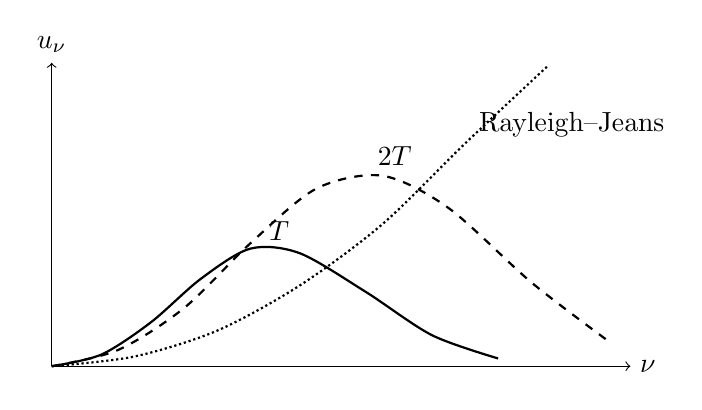
\begin{tikzpicture}[x=1.05cm,y=0.82cm]
\draw[->] (0,0)--(7.0,0) node[right] {\(\nu\)};
\draw[->] (0,0)--(0,4.7) node[above] {\(u_\nu\)};
\draw[densely dotted,thick] plot[smooth] coordinates
  {(0,0) (1,0.15) (2,0.55) (3,1.25) (4,2.20) (5,3.45) (6,4.65)};
\draw[thick] plot[smooth] coordinates
  {(0,0) (0.6,0.18) (1.2,0.68) (1.8,1.35) (2.4,1.82) (3.0,1.75) (3.8,1.15) (4.6,0.48) (5.4,0.12)};
\draw[thick,dashed] plot[smooth] coordinates
  {(0,0) (0.8,0.25) (1.6,0.90) (2.4,1.90) (3.2,2.75) (4.0,2.95) (4.8,2.45) (5.8,1.30) (6.7,0.42)};
\node[anchor=west] at (5.05,3.75) {Rayleigh--Jeans};
\node at (2.75,2.10) {\(T\)};
\node at (4.15,3.25) {\(2T\)};
\end{tikzpicture}
\caption{El espectro clásico crece sin límite, mientras que los espectros de Planck alcanzan un máximo y luego caen. Al aumentar la temperatura, la frecuencia característica se desplaza hacia valores más altos y se conserva la forma adimensional.}
\label{fig:c07-planck-redraw}
\end{figure}

La inmensa mayoría de los fotones del universo actual pertenecen al fondo de microondas y tienen una longitud de onda característica del orden de un milímetro. La ecuación~\eqref{eq:c07-thermal-wavelength} relaciona esa longitud de onda con unos pocos kelvin, que aquí se redondean convencionalmente a \(3\,\mathrm{K}\). Una longitud de onda por sí sola solo permitiría establecer una relación aproximada. La evidencia más sólida es que las mediciones en muchas frecuencias trazan la curva completa de cuerpo negro con gran precisión.

\begin{classroomqa}
\audiencequestion{¿Qué espacio ocupa un fotón del fondo cósmico de microondas?}
\lecturerresponse{Un fotón no tiene un tamaño definido y universal. Puede prepararse como un paquete de ondas cuya extensión espacial depende del estado, mientras que su longitud de onda fija la escala de sus oscilaciones. En el fondo térmico, tanto la longitud de onda característica como una escala natural del paquete de ondas son del orden de un milímetro, pero ninguna debe confundirse con el radio de un pequeño objeto clásico. \lecturetimestamp{00:57:16--00:59:05}}
\end{classroomqa}

\section{La expansión congela la forma de cuerpo negro}

Empecemos con una caja caliente que contiene hidrógeno ionizado y radiación en equilibrio. Al expandirse la caja, su contenido realiza trabajo, la densidad de energía disminuye y la temperatura baja. Finalmente, los electrones y los protones permanecen unidos en forma de átomos neutros. La formación de átomos se llama \emph{recombinación}; la pérdida de la dispersión eficaz entre fotones y --materia se llama \emph{desacoplamiento}. Ambos procesos están estrechamente relacionados, pero sus nombres designan sucesos físicos distintos.

Tras el desacoplamiento, la materia y la radiación ya no comparten una temperatura común. Sin embargo, el espectro de los fotones conserva su forma de Planck. Todas las longitudes de onda que se propagan libremente se estiran por el mismo factor de expansión,
\begin{equation}
\lambda\propto a,
\qquad
\nu\propto a^{-1}.
\end{equation}
Como la curva de Planck depende de \(\nu/T\), este corrimiento al rojo uniforme equivale a asignar a la radiación una temperatura
\begin{equation}
\boxed{T_\gamma\propto a^{-1}.}
\label{eq:c07-temperature-scaling}
\end{equation}
Así, la expansión conserva la forma aunque ya no haya colisiones que la reconstruyan continuamente. La materia sigue su propia historia térmica posterior.

Por tanto, el fondo de microondas observado es un vestigio de una distribución en equilibrio. Su forma de cuerpo negro se estableció cuando las cargas libres dispersaban con eficiencia y luego se conservó mediante el corrimiento al rojo cosmológico uniforme. Existen la luz de las estrellas, los rayos gamma y otras fuentes posteriores, pero su número es pequeño frente a la población de fotones relictos y sus orígenes astrofísicos se pueden identificar.

\begin{classroomqa}
\audiencequestion{¿Cómo puede la radiación conservar su forma de cuerpo negro cuando deja de estar en equilibrio con la materia?}
\lecturerresponse{Las colisiones son necesarias para crear el espectro de equilibrio, pero no para conservarlo bajo una expansión perfectamente uniforme. Multiplicar todas las longitudes de onda por el mismo factor transforma un espectro de Planck en otro de menor temperatura. Los fotones dejan de compartir la temperatura de la materia, pero conservan su propia temperatura de cuerpo negro.}
\end{classroomqa}

\section{Por qué la recombinación ocurre tan tarde}

La longitud de onda actual y la longitud de onda en el desacoplamiento están relacionadas por
\begin{equation}
\frac{\lambda_0}{\lambda_{\rm dec}}
=
\frac{a_0}{a_{\rm dec}}
=
\frac{T_{\rm dec}}{T_0}.
\label{eq:c07-decoupling-ratio}
\end{equation}
El desacoplamiento no es matemáticamente instantáneo, pero es suficientemente breve en comparación con la historia posterior como para asignarle un factor de escala y una temperatura característicos. Aquí, \(T_0\) denota la temperatura del CMB, no la temperatura cinética de la materia intergaláctica.

La energía de ionización del estado fundamental del hidrógeno es
\begin{equation}
\chi_H=13.6\,\mathrm{eV}.
\end{equation}
Una primera estimación consistiría en tomar \(k_BT\sim\chi_H\), de modo que un fotón típico pudiera ionizar un átomo. Esa estimación da una temperatura demasiado alta, porque un espectro térmico contiene una cola de alta energía y el universo contiene un número enorme de fotones.

\begin{figure}[htbp]
\centering
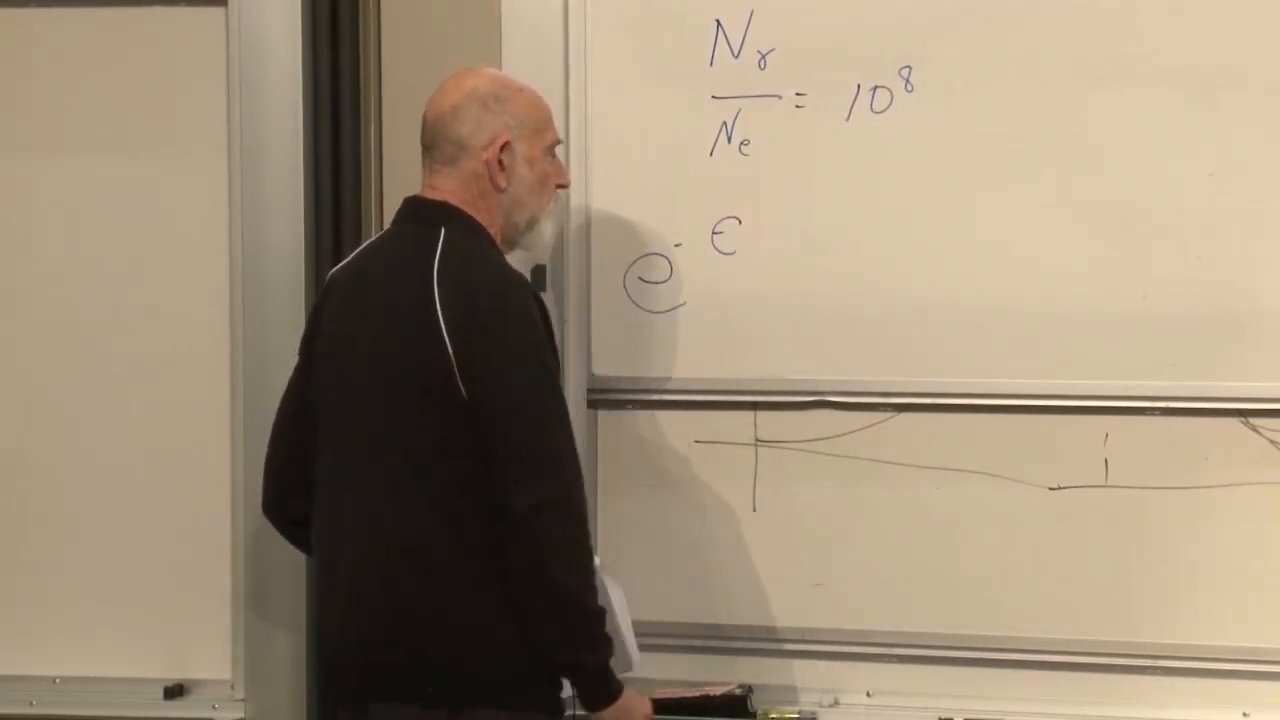
\includegraphics[width=0.82\textwidth]{lecture_07_figure_03.png}
\caption{La pizarra introduce la razón de abundancias observada \(N_\gamma/N_e=10^8\) y el símbolo de la energía de los fotones \(\epsilon\). Solo se ve el comienzo del exponente; el factor de Boltzmann completo se obtiene a partir de la derivación oral.}
\label{fig:c07-boltzmann-board}
\lectureframe{01:06:10.631}
\end{figure}

La razón de abundancias redondeada que se usa aquí es
\begin{equation}
\frac{N_\gamma}{N_e}\sim10^8.
\label{eq:c07-photon-electron-ratio}
\end{equation}
Se infiere al comparar la densidad medida de fotones del CMB con el contenido de materia ordinaria. Para una energía de fotón \(\epsilon\), la cola de alta energía tiene la forma de Boltzmann
\begin{equation}
P(\epsilon)\propto e^{-\epsilon/(k_BT)}.
\end{equation}
Por tanto, se estima que el número de fotones ionizantes disponibles por átomo es
\begin{equation}
10^8 e^{-\chi_H/(k_BT)}.
\end{equation}
La ionización sigue siendo eficaz hasta que esta cantidad cae a un valor del orden de la unidad.

Al tomar logaritmos se obtiene
\begin{equation}
\frac{\chi_H}{k_BT}
\sim
\ln 10^8
\simeq18.4,
\end{equation}
o, con la precisión pretendida,
\begin{equation}
k_BT\sim\frac{\chi_H}{20}.
\label{eq:c07-tail-estimate}
\end{equation}
El fotón característico puede tener una energía muy inferior al umbral porque basta un fotón ionizante de la cola por átomo.

\begin{classroomqa}
\audiencequestion{¿La estimación de la cola cuenta los fotones que están justo en el umbral o todos los que lo superan?}
\lecturerresponse{Cuenta los fotones con energía igual o superior al umbral. Como la cola decrece exponencialmente, la mayor parte de esa integral proviene de energías cercanas a \(\chi_H\), así que la estimación exponencial sencilla recoge el orden de magnitud pertinente. \lecturetimestamp{01:08:39--01:08:54}}
\end{classroomqa}

\begin{classroomqa}
\audiencequestion{¿La razón \(N_\gamma/N_e\) también era aproximadamente \(10^8\) en el momento del desacoplamiento?}
\lecturerresponse{Con la aproximación usada aquí, sí. Desde el desacoplamiento hasta épocas mucho más calientes, la expansión diluye ambas poblaciones por el mismo factor de volumen y no crea ni destruye cantidades suficientes de ninguna de las dos especies como para alterar su razón. A temperaturas aún mayores, las reacciones de producción de pares exigen llevar una contabilidad nueva. \lecturetimestamp{01:08:54--01:09:57}}
\end{classroomqa}

\begin{classroomqa}
\audiencequestion{¿Los fotones emitidos por las estrellas contribuyen de manera apreciable a este recuento?}
\lecturerresponse{No. Las estrellas aún no existían en la época de la recombinación e incluso hoy sus fotones son una fracción diminuta de la población del CMB. La razón de la ecuación~\eqref{eq:c07-photon-electron-ratio} se refiere a los fotones térmicos relictos. \lecturetimestamp{01:11:44--01:12:39}}
\end{classroomqa}

\begin{classroomqa}
\audiencequestion{Cuando los electrones se recombinan con los protones, ¿no deberían los fotones emitidos dejar una característica espectral nítida del hidrógeno en el espectro de cuerpo negro?}
\lecturerresponse{Mientras la dispersión y la absorción sean rápidas en comparación con la expansión, la radiación se reprocesa continuamente y se mantiene cerca del equilibrio térmico. Una congelación suficientemente abrupta podría conservar una distorsión, pero la recombinación lenta y cercana al equilibrio impide que una línea aislada de gran intensidad sustituya a la forma de cuerpo negro. \lecturetimestamp{01:12:42--01:14:07}}
\end{classroomqa}

La estimación resultante de nivel introductorio es \(T_{\rm dec}\sim4\times10^3\,\mathrm{K}\). Una conversión directa de \(\chi_H/20\) da un valor algo mayor, lo que lleva a sugerir que el denominador efectivo quizá esté más cerca de \(40\). No hay contradicción; esto pone de manifiesto lo burdo que es sustituir todo el equilibrio de ionización por un único recuento de la cola. Un tratamiento controlado del equilibrio emplea la relación de Saha,
\begin{equation}
\frac{x_e^2}{1-x_e}
=
\frac{1}{n_H}
\left(\frac{m_e k_BT}{2\pi\hbar^2}\right)^{3/2}
e^{-\chi_H/(k_BT)},
\label{eq:c07-saha}
\end{equation}
y después la cinética de recombinación fuera del equilibrio. El argumento aproximado es útil porque identifica la física dominante: la diminuta razón de bariones a fotones retrasa la supervivencia de los átomos neutros hasta una temperatura muy inferior a \(\chi_H/k_B\).

\section{Corrimiento al rojo hasta la superficie de última dispersión}

Con \(T_0\simeq3\,\mathrm{K}\) y \(T_{\rm dec}\sim4\times10^3\,\mathrm{K}\), la ecuación~\eqref{eq:c07-decoupling-ratio} da
\begin{equation}
\boxed{
\frac{a_0}{a_{\rm dec}}
\sim
\frac{T_{\rm dec}}{T_0}
\sim10^3
}.
\label{eq:c07-decoupling-expansion}
\end{equation}
De manera equivalente, el corrimiento al rojo de la última dispersión es del orden de \(10^3\). Antes de esta época, el plasma ionizado era opaco; después, los fotones se propagaron casi libremente.

Este suceso térmico ocurrió apenas unos cientos de miles de años después del comienzo de la expansión caliente; en el intercambio se cita convencionalmente un valor aproximado de \(380{,}000\) años. Ese intervalo es ínfimo comparado con la edad cósmica posterior. Desde el desacoplamiento, las longitudes han aumentado aproximadamente \(10^3\) veces y los elementos de volumen comóvil, aproximadamente \(10^9\) veces.

El desacoplamiento es un hito térmico, pero no el único suceso de la historia intermedia. La formación de galaxias, estrellas y agujeros negros ocurre más tarde, pero aquí se deja de lado para poder seguir con claridad los hitos térmicos hacia el pasado.

Mirar hacia el exterior es mirar hacia el pasado. Las capas cercanas muestran épocas recientes; las más lejanas muestran épocas anteriores. Nuestro cono de luz pasado acaba encontrándose con la época de recombinación, y la intersección con esa época es la superficie de última dispersión. Antes, la radiación electromagnética se dispersaba repetidamente con las cargas libres y no podía viajar directamente hasta nosotros.

\begin{figure}[htbp]
\centering
\begin{coursefitfigure}
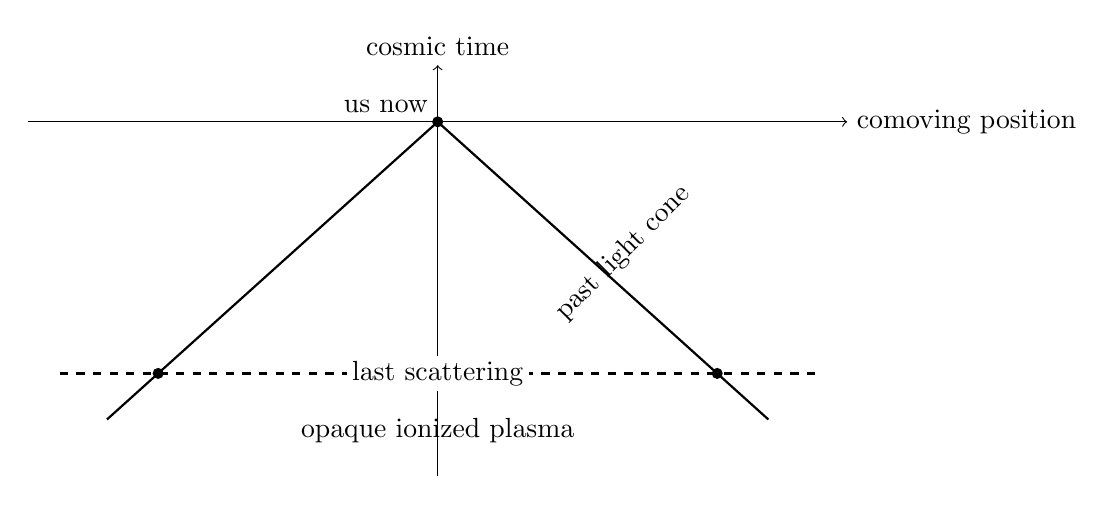
\begin{tikzpicture}[x=1.0cm,y=0.9cm]
\draw[->] (0,0)--(0,5.8) node[above] {cosmic time};
\draw[->] (-5.2,5.0)--(5.2,5.0) node[right] {comoving position};
\draw[thick] (0,5.0)--(-4.2,0.8);
\draw[thick] (0,5.0)--(4.2,0.8);
\draw[thick,dashed] (-4.8,1.45)--(4.8,1.45);
\fill (0,5.0) circle (2pt) node[above left] {us now};
\fill (-3.55,1.45) circle (2pt);
\fill (3.55,1.45) circle (2pt);
\node[fill=white,inner sep=2pt] at (0,1.45) {last scattering};
\node at (0,0.65) {opaque ionized plasma};
\node[rotate=45] at (2.35,3.15) {past light cone};
\end{tikzpicture}
\end{coursefitfigure}
\caption{La observación electromagnética retrocede por el cono de luz pasado solo hasta la superficie de última dispersión. Antes, el plasma ionizado dispersaba los fotones repetidamente.}
\label{fig:c07-last-scattering}
\end{figure}

\begin{classroomqa}
\audiencequestion{¿El desacoplamiento pone fin a toda posible observación de épocas anteriores?}
\lecturerresponse{Pone fin a la observación electromagnética directa, porque el plasma era opaco a los fotones. Otros mensajeros que interactúan más débilmente podrían haber escapado antes: en principio, los neutrinos relictos permiten sondear una capa más profunda y la radiación gravitacional podría aportar información de épocas aún anteriores. Por tanto, gran parte de nuestro conocimiento sobre lo ocurrido antes de la última dispersión es indirecto, pero no arbitrario. \lecturetimestamp{01:32:27--01:36:31}}
\end{classroomqa}

\begin{classroomqa}
\audiencequestion{¿Cuál era el valor absoluto de \(a\) al comienzo, y era necesariamente el universo un objeto diminuto y finito?}
\lecturerresponse{En un espacio plano, solo las razones entre factores de escala tienen significado invariante; la normalización de \(a\) es arbitraria. Una sección espacial con curvatura negativa también puede ser infinita. Un universo cerrado \(k=+1\) tiene un radio de curvatura finito, pero las observaciones determinan razones de expansión y no un tamaño primordial conocido. El big bang caliente no implica, por sí solo, que todo el espacio fuera una pequeña esfera. \lecturetimestamp{01:30:05--01:32:22}}
\end{classroomqa}

\begin{classroomqa}
\audiencequestion{Como el CMB es más antiguo que las galaxias, ¿verlo nos permite saber si existen galaxias hoy más allá de nuestra región observable?}
\lecturerresponse{No. El CMB muestra una región lejana tal como era en el momento del desacoplamiento, no tal como es hoy. La luz de galaxias actuales suficientemente lejanas no ha tenido tiempo de llegar hasta nosotros. La continuidad de las poblaciones de galaxias más allá de nuestro horizonte se apoya en la homogeneidad observada a gran escala y en la ausencia de un borde visible, no en una observación directa proporcionada por el CMB. \lecturetimestamp{01:59:01--02:00:58}}
\end{classroomqa}

La cronología resultante retrocede desde el presente, pasa por la formación de galaxias y el desacoplamiento, y llega a la igualdad entre materia--radiación. Aún antes, la disminución del factor de escala implica un aumento de la temperatura y la aparición de nuevas especies de partículas.

\section{Igualdad entre materia--radiación}

Al retroceder más allá del desacoplamiento aparece otro hito. La materia no relativista y la radiación se diluyen de forma distinta:
\begin{equation}
\rho_m\propto a^{-3},
\qquad
\rho_r\propto a^{-4},
\qquad
\frac{\rho_m}{\rho_r}\propto a.
\label{eq:c07-equality-scaling}
\end{equation}
La materia domina en épocas tardías, pero la radiación necesariamente domina cuando \(a\) es suficientemente pequeño. La ley de expansión cambia en consecuencia del comportamiento de la era dominada por materia, \(a\propto t^{2/3}\), al comportamiento de la era dominada por radiación, \(a\propto t^{1/2}\).

Una estimación deliberadamente aproximada parte de \(10^8\) fotones por protón, una energía característica de los fotones del CMB de \(10^{-4}\,\mathrm{eV}\) y una energía de reposo del protón de \(10^9\,\mathrm{eV}\). Si se ignora la materia oscura, se obtiene
\begin{equation}
\left(\frac{\rho_m}{\rho_r}\right)_0
\sim
\frac{10^9}{10^8\,10^{-4}}
\sim10^5.
\end{equation}
Luego se corrige el argumento: la materia oscura aporta mucha más masa que los bariones luminosos, con lo que la estimación redondeada pasa a ser \(10^6\). Con esta aritmética, la ecuación~\eqref{eq:c07-equality-scaling} sitúa la igualdad en
\begin{equation}
\frac{a_{\rm eq}}{a_0}\sim10^{-6},
\qquad
\frac{T_{\rm eq}}{T_0}\sim10^6.
\label{eq:c07-equality-estimate}
\end{equation}
Son estimaciones introductorias para fijar escalas, no un ajuste preciso de los parámetros cosmológicos. Su propósito es mostrar cómo potencias distintas de \(a\) sitúan las sucesivas eras térmicas.

La era dominada por la radiación queda detrás de la barrera de última dispersión electromagnética, pero su existencia se deduce de las densidades medidas en épocas tardías y de las leyes de escala conocidas. Al continuar hacia temperaturas más altas, tarde o temprano deja de ser válida la suposición de que los números de protones, electrones y fotones se conservan por separado, porque las colisiones energéticas empiezan a crear pares de partículas--antipartículas masivas.

\begin{classroomqa}
\audiencequestion{¿La afirmación de que se conservan los números de fotones y protones incluye la luz de las estrellas y temperaturas arbitrariamente altas?}
\lecturerresponse{No. Se aplica a la población relicta del CMB durante el intervalo en que las reacciones que cambian el número de partículas son ineficaces. La luz de las estrellas se creó más tarde y es insignificante en el recuento de fotones. A temperaturas suficientemente altas, la creación de pares cambia el contenido de partículas y deja de cumplirse la conservación de cada número por separado. La recombinación misma añade, como máximo, aproximadamente un fotón por electrón: solo una parte en \(10^8\) de la población de fotones del CMB ya existente. \lecturetimestamp{01:26:24--01:27:40}}
\end{classroomqa}

\section{Creación de pares y la sopa casi simétrica}

A una temperatura del orden de
\begin{equation}
T\sim10^{10}\,\mathrm{K},
\qquad
\frac{a_0}{a}\sim10^{14},
\end{equation}
la energía característica de los fotones es de alrededor de un megaelectronvoltio, comparable a la escala de energía de reposo necesaria para crear un par electrón--positrón. Entonces, dos fotones pueden reaccionar mediante
\begin{equation}
\gamma+\gamma
\longleftrightarrow
e^-+e^+.
\label{eq:c07-pair-reaction}
\end{equation}
El umbral exacto depende de la cinemática de la colisión, pero la energía de reposo del electrón, \(m_ec^2\), fija la escala pertinente.

La creación y la aniquilación de pares se equilibran rápidamente. Si hay muy pocos pares, las colisiones de fotones los reponen; si hay demasiados, la aniquilación devuelve su energía a los fotones. Por tanto, las abundancias de fotones, electrones y positrones quedan determinadas por la temperatura y son todas del mismo orden en el plasma relativista. Ya no conservan un recuerdo sencillo de sus números posteriores.

\begin{classroomqa}
\audiencequestion{¿Cómo puede mantenerse eléctricamente neutro este plasma lleno de pares si ya hay electrones que compensan a los protones?}
\lecturerresponse{Cada reacción crea una carga negativa y otra positiva, así que los pares no añaden carga neta. Constituyen una población enorme y casi simétrica superpuesta a un pequeño exceso de electrones. Los electrones individuales son indistinguibles; solo la diferencia \(N_{e^-}-N_{e^+}\) conserva el recuerdo de la carga necesaria para compensar la de los protones. \lecturetimestamp{01:42:31--01:43:14}}
\end{classroomqa}

Las reacciones de pares cambian la suma, pero conservan la diferencia:
\begin{equation}
N_{e^-}+N_{e^+}\quad\hbox{changes},
\qquad
N_{e^-}-N_{e^+}=\hbox{constant}.
\label{eq:c07-pair-invariants}
\end{equation}
En la sopa caliente, \(N_{e^-}+N_{e^+}\) es del mismo orden que \(N_\gamma\), mientras que el exceso superviviente es del mismo orden que el número, mucho menor, de protones. Por tanto, la razón redondeada es
\begin{equation}
\boxed{
\frac{N_{e^-}-N_{e^+}}
{N_{e^-}+N_{e^+}}
\sim10^{-8}
}.
\label{eq:c07-asymmetry}
\end{equation}
Había aproximadamente un electrón excedente por cada \(10^8\) pares electrón--positrón.

Esto invierte la pregunta original. El hecho sorprendente no es simplemente que haya muchos fotones. A temperaturas altas, los fotones y los pares tienen abundancias naturalmente comparables. El enigma es por qué las poblaciones de partículas negativas y positivas difieren y por qué su diferencia relativa es diminuta, en vez de ser exactamente cero o del orden de la unidad. Un estado inicial simétrico y una producción simétrica de pares no producirían ningún exceso. El origen microscópico de la asimetría no nula es el problema que se abordará en la siguiente etapa de la discusión.

A temperaturas dos o tres órdenes de magnitud más altas, ya no se puede ignorar la estructura del protón. Las colisiones producen quarks y antiquarks, mientras que los protones se disuelven en sus constituyentes; fotones, leptones, quarks, antiquarks, gluones y las especies oscuras suficientemente ligeras forman un plasma más caliente. Allí la energía del vacío es dinámicamente despreciable, porque la densidad de radiación aumenta como \(a^{-4}\).

El exceso correspondiente de quarks está ligado al exceso de electrones por la neutralidad de la carga total. Tres quarks de valencia forman un barión, de modo que la contabilidad difiere en factores convencionales, pero la materia bariónica superviviente y los electrones supervivientes no son desequilibrios de carga independientes. Su pequeñez común es una reliquia del universo temprano.

Sigamos de nuevo la evolución del plasma de electrones--positrones. Cuando la temperatura cae por debajo de la escala de producción de pares, la aniquilación continúa mientras la reacción inversa se vuelve infrecuente. Casi todos los electrones encuentran un positrón, la energía de los pares se convierte en radiación y solo queda la diminuta población sobrante de electrones. La materia que nos rodea es este desequilibrio residual, no una muestra representativa de la enorme población de pares que hubo una vez.

\begin{classroomqa}
\audiencequestion{¿Qué hacían los protones durante la era de aniquilación de pares electrón--positrón?}
\lecturerresponse{En esa etapa, la temperatura era lo bastante alta para crear pares de electrones, pero todavía no para crear cantidades abundantes de pares protón--antiprotón ni para disolver protones en quarks. Por tanto, la población de protones era pequeña pero persistente, y la neutralidad exigía \(N_{e^-}-N_{e^+}\simeq N_p\). \lecturetimestamp{01:55:35--01:56:53}}
\end{classroomqa}

El universo visible parece presentar el mismo signo de exceso de materia en todas partes. La evidencia expuesta en clase es la ausencia de antinúcleos en los rayos cósmicos: las colisiones secundarias pueden producir antiprotones ocasionales, pero cabría esperar que una antigalaxia aportara antinúcleos complejos. Este es un argumento observacional propio de la época de la conferencia, no una afirmación de que se hayan inspeccionado regiones más allá del horizonte observable.

\begin{classroomqa}
\audiencequestion{¿Podría el exceso observado de materia ser una fluctuación local, con regiones de antimateria más allá de lo que podemos ver?}
\lecturerresponse{El mismo signo en el enorme volumen observable es demasiado coherente para deberse a una fluctuación aleatoria. Hace falta una explicación dinámica. Sin embargo, más allá de la región observable no se dispone de evidencia directa; no se puede descartar una transición a un dominio diferente por el mero hecho de observar más allá de donde ha llegado la luz. \lecturetimestamp{01:56:57--01:58:47}}
\end{classroomqa}

\begin{classroomqa}
\audiencequestion{¿Es ya la explicación de materia--antimateria una teoría numérica precisa, y se produce la unificación de las fuerzas a esta temperatura?}
\lecturerresponse{Existe una teoría cualitativa de cómo puede surgir una pequeña asimetría, pero aquí no se deriva el valor redondeado \(10^{-8}\) a partir de un modelo microscópico único. La unificación de las fuerzas corresponde a temperaturas mucho más altas que las de la época de los pares de electrones. Ambas preguntas requieren física que va más allá de los hitos térmicos actuales. \lecturetimestamp{01:51:36--01:52:24}}
\end{classroomqa}

\section{Qué conviene recordar}

La historia térmica se organiza en torno a tasas y umbrales. La dispersión rápida establece una temperatura común; la formación de átomos neutros elimina los dispersores; después, la expansión uniforme desplaza al rojo un espectro de Planck congelado sin alterar su forma. Por tanto, el CMB es a la vez un termómetro de la radiación y una superficie visible que marca el fin del acceso electromagnético directo al plasma anterior.

El exceso de fotones convierte la recombinación en un problema de cola, no de energía media. La escala \(T_{\rm dec}/T_0\sim10^3\) sitúa la última dispersión, mientras que las distintas leyes de dilución de la materia y la radiación sitúan una época anterior de igualdad. A temperaturas aún más altas, la creación de pares borra la memoria del número total de electrones y positrones, pero conserva su diminuta diferencia. Esa asimetría residual, reflejada en el sector bariónico, es el dato inicial inexplicado al que debe enfrentarse la siguiente investigación.
